\documentclass{article}

% Margins
\topmargin=-0.45in
\evensidemargin=0in
\oddsidemargin=0in
\textwidth=6.5in
\textheight=9.0in
\headsep=0.25in 

\linespread{1.1} % Line spacing

% Set up the header and footer
%\pagestyle{fancy}

\setlength\parindent{0pt} % Removes all indentation from paragraphs
\usepackage[utf8]{inputenc}
\usepackage[T1]{fontenc}
\usepackage{graphicx}
\usepackage{float}

\usepackage[spanish]{babel} % Español como idioma principal del texto (permite hyphenation de palabras al final de una línea)
\selectlanguage{spanish}
\usepackage{hyperref}
\graphicspath{{Diagrams/export/}{Diagrams/static/export_pdf/}}

\begin{document}
\title{MarcoPolo}
\author{Diego Martín}
\maketitle

\section{Introducción}

\section{Objetivos del sistema}

Se definen a continuación los objetivos del sistema a alto nivel:

\section{Requisitos no funcionales}

\subsection{Independencia}

La implementación del protocolo debe ser independiente de las aplicaciones que lo utilizarán, a fin de poder aumentar la adaptabilidad del protocolo a nuevas situaciones. Dicho objetivo se consigue delegando una gran parte de la funcionalidad a aplicaciones que se apoyan sobre esta implementación, en vez de albergar dicha funcionalidad en la misma.

\subsection{\textit{Zeroconf}}

El protocolo funciona en una red sin requerir ningún tipo de configuración por parte del usuario, y en la mayoría de casos sin gran esfuerzo por parte del administrador.

\subsection{Segmentación}

Varias instancias del protocolo pueden ejecutarse en una misma red de forma independiente, permitiendo la creación de varias ``mallas'' de equipos. Dicha segmentación no debe alterar en absoluto el esquema de la red preexistente.

\subsection{Conectable}

Las diferentes aplicaciones presentes en los diferentes nodos deben poder aprovechar la funcionalidad del protocolo mediante una serie de elementos conectores (\textit{bindings}).

\subsection{Seguridad}

En aquellos casos en los que la información enviada a través de los \textit{bindings} o compartida por los nodos sea confidencial, el protocolo debe implementar las medidas oportunas para la protección de la misma.

\subsection{Independencia de plataforma e implementación}

Toda la comunicación entre elementos del protocolo se realizará a través de tecnologías que no dependan de una implementación concreta, tales como un lenguaje de programación o un sistema operativo dado. El único elemento que puede presentar tal dependencia es el conector final con otro código fuente, así como cualquier otro punto final (comandos, ficheros de configuración, etc).

\subsection{Independencia del espacio de direcciones, nombres o cualquier otro elemento de red}

El protocolo debe funcionar en cualquier espacio de direcciones dado, sin considerar en cualquier caso la dependencia con protocolos como \textbf{DHCP} o \textbf{DNS}.

\subsection{Simplicidad}

Los comandos del protocolo deben ser simples y, en caso de que sea posible, deben ser similares a otros ya conocidos por los usuarios del sistema, a fin de que estos ya estén familiarizados con los mismos.

\subsection{Descentralización}

El protocolo no debe en ningún momento establecer un potencial ``cuello de botella''.

\subsection{Configurable}

\subsection{Visibilidad}

\subsection{Optimización de la red}

\subsection{Sin conexión}

\subsection{Extensible}

\subsection{Extensible a diferente hardware}

\section{Protocolo}

\subsection{Marco}


\section{Propuesta de implementación}

\subsection{Vista estática}

\begin{figure}[H]
\centering
\includegraphics[width=0.6\textwidth]{Paquetes}
\end{figure}

\subsubsection{Paquete Marco}

\begin{figure}[H]
\centering
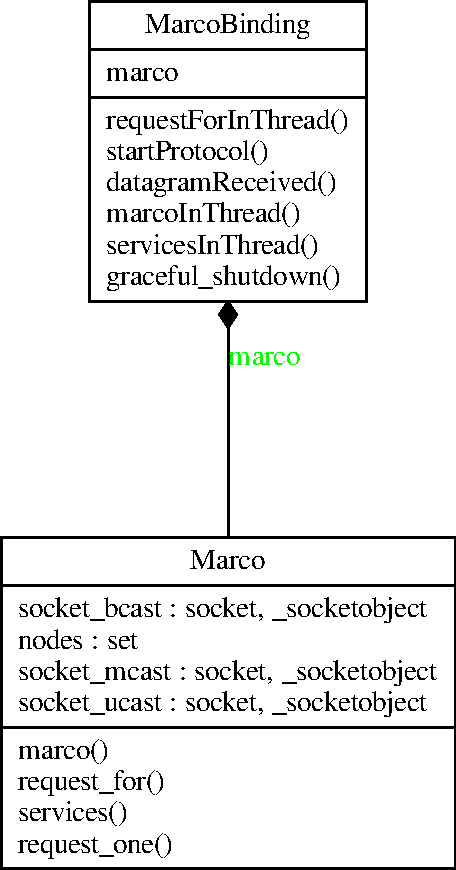
\includegraphics[width=0.2\textwidth]{class_marco_marcobinding}
\end{figure}

\begin{figure}[H]
\centering

\includegraphics[width=0.2\textwidth]{class_marcoexception}
\end{figure}

\subsubsection{Paquete Polo}

\begin{figure}[H]
\centering
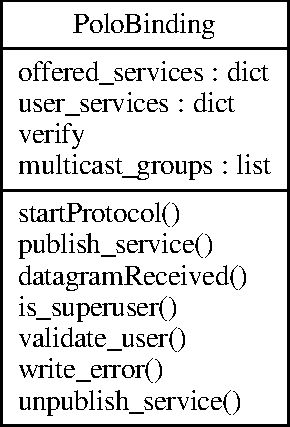
\includegraphics[width=0.2\textwidth]{class_polobinding}
\end{figure}

\begin{figure}[H]
\centering
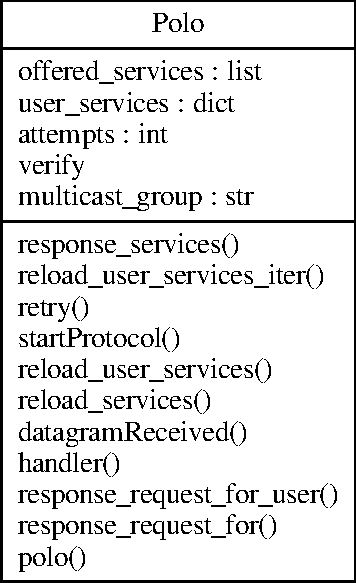
\includegraphics[width=0.2\textwidth]{class_polo}
\end{figure}


\subsubsection{Paquete utils}

\begin{figure}[H]
\centering
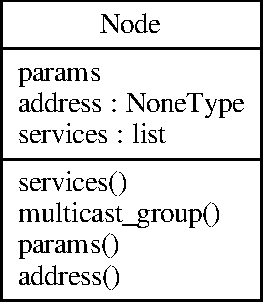
\includegraphics[width=0.2\textwidth]{class_node}
\end{figure}

\subsubsection{Paquete tests}

\begin{figure}[H]
\centering
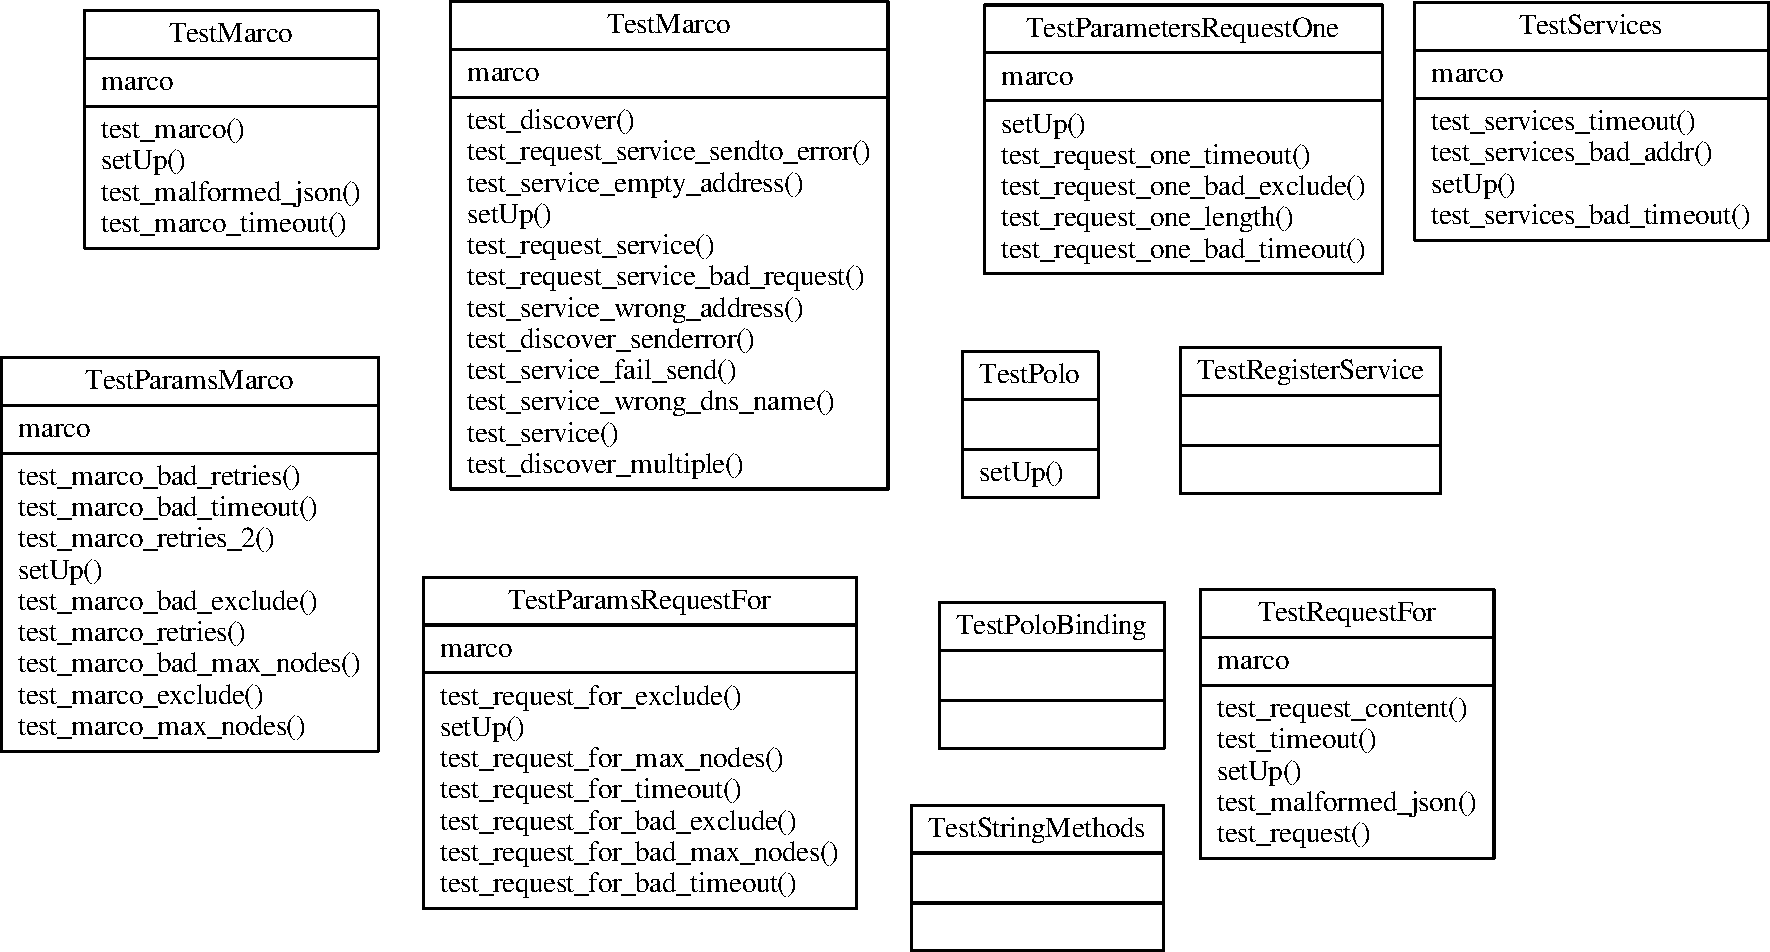
\includegraphics[width=0.2\textwidth]{classes_test}
\end{figure}

\subsection{Vista de interacción}

\subsubsection{Diagramas de comunicación}

\paragraph{Comunicación en Marco}

\begin{figure}[H]
\centering
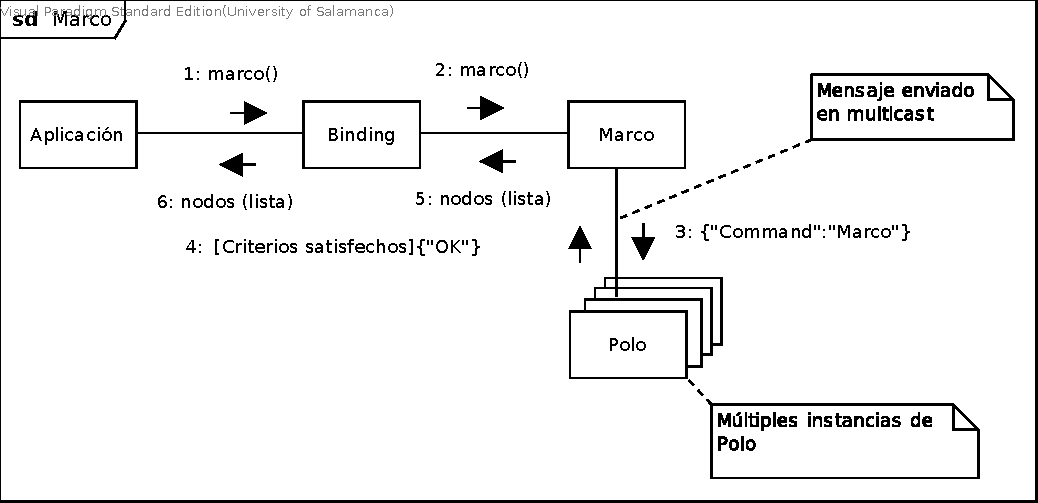
\includegraphics[width=0.6\textwidth]{Marco}
\end{figure}

\paragraph{Comunicación en Polo}

\begin{figure}[H]
\centering
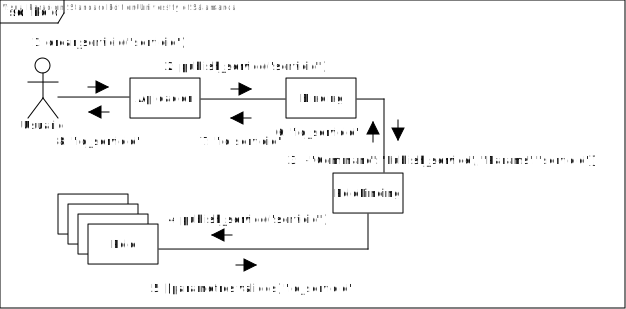
\includegraphics[width=0.6\textwidth]{Polo}
\end{figure}

\subsection{Vista de actividad}

\begin{figure}[H]
\centering
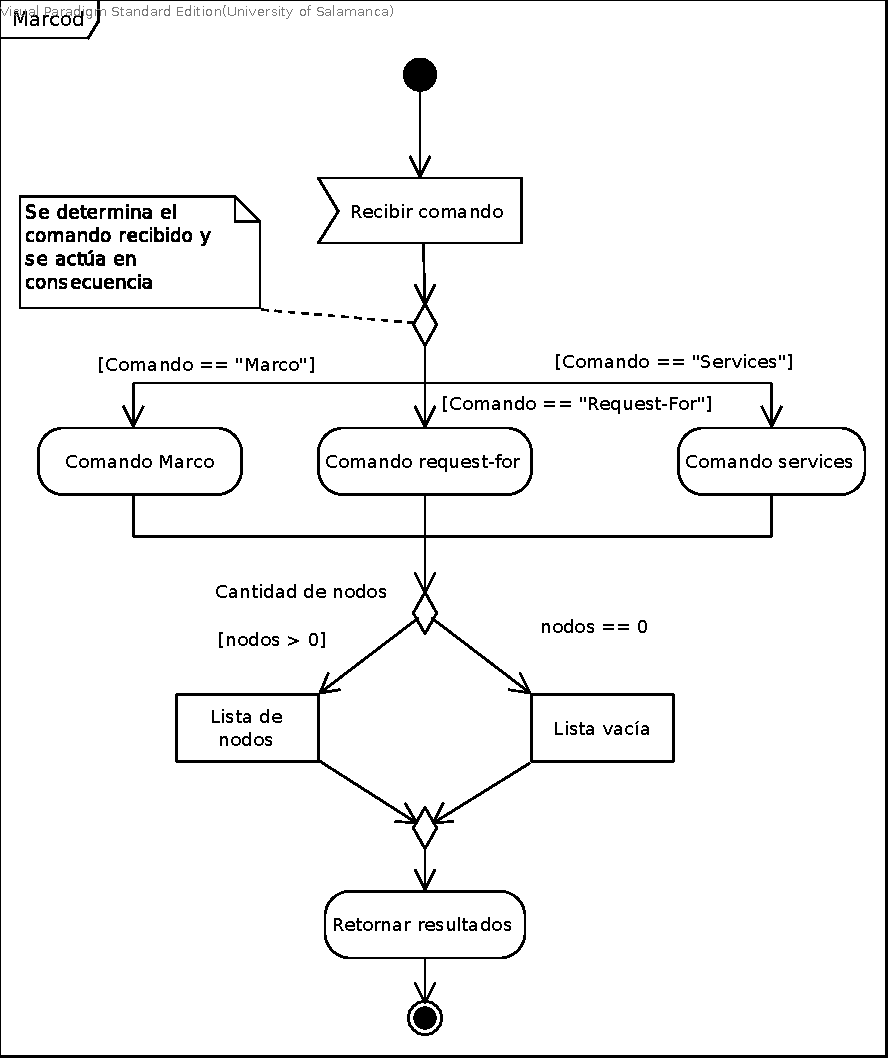
\includegraphics[width=0.7\textwidth]{Marcod}
\end{figure}

\begin{figure}[H]
\centering
\includegraphics[width=0.7\textwidth]{Comando_Marco}
\end{figure}

\end{document}